\documentclass[]{article}
\usepackage{xcolor}
\usepackage{listings}
\usepackage{showexpl}
\usepackage[bahasai]{babel}
\usepackage{graphicx}
\lstset{language=C++,
	% numbers=left,
	%	stepnumber=1,
	numberstyle=\ttfamily,
	basicstyle=\ttfamily,
	keywordstyle=\color{blue}\ttfamily,
	stringstyle=\color{red}\ttfamily,
	commentstyle=\color{gray}\ttfamily,
	morecomment=[l][\color{magenta}]{\#}
}


%opening
\title{Tugas 2: Implementasi Struktur Pada Array}
\author{Akhmad Thoriq Afif NRP 5024201028}

\begin{document}
\maketitle
\section{Listing Program}
Berikut ini merupakan source code dari tugas 2 Implementasi Struktur pada Array. Program ini dibuat dengan bahasa pemrograman C++.
\lstinputlisting[label={kodingan},caption={Implementasi Struktur pada Array}, language={C++}]{tugas.cpp}
\subsection*{OUTPUT PROGRAM:}
% add graphics
\begin{figure}[htp]
    \centering
    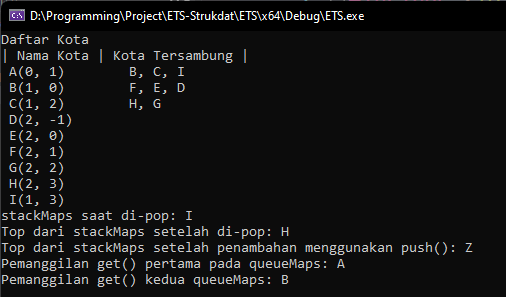
\includegraphics[width=8cm]{output.png}
    \caption{Output Program}
    \label{fig:galaxy}
\end{figure}
\pagebreak
\section{Penjelasan Program}
\subsection{Desain struktur data}
\par
Pada program ini terdapat struct Node yang merupakan representasi dari Kota. Dalam Node ini terdapat atribut nama kota, kota yang tersambung, dan koordinat kota. Selain Node, terdapat class Maps. Class Maps menyimpan Node-Node yang ada. Node tersebut disimpan kedalam sebuah array yang dapat ditentukan ukurannya.
\subsection{Fungsi untuk menambah kota}
\lstinputlisting[label={maxvalue},caption={Fungsi untuk menambah kota}, language={C++}, firstline=99, lastline=112]{tugas.cpp}
\par
Fungsi ini digunakan untuk menambahkan kota. Dibutuhkan 3 parameter yaitu nama kota dan koordinat kota. Langkah-langkah dalam menambah kota adalah sebagai berikut:
\begin{enumerate}
    \item Membuat object Node baru bernama newCity.
    \item Melakukan pengecekan ukuran Maps. Jika ukuran Maps masih cukup maka akan dilakukan penambahan kota.
\end{enumerate}
\subsection{Fungsi untuk menghapus kota}
\lstinputlisting[label={hapusmaks},caption={Fungsi untuk menghapus kota}, language={C++}, firstline=114, lastline=127]{tugas.cpp}
\par
Fungsi ini digunakan untuk menghapus kota. Dibutuhkan 1 parameter yaitu nama kota. Langkah-langkah dalam menghapus kota adalah sebagai berikut:
\begin{enumerate}
    \item Melakukan pencarian index kota yang akan dihapus dengan menggunakan fungsi findCityByname.
    \item Memindahkan elemen sebelah kanan kota yang akan dihapus ke index kota yang akan dihapus.
    \item Mengurangi ukuran Maps.
\end{enumerate}
\subsection{Fungsi untuk mencari kota}
\lstinputlisting[label={findcitybynama},caption={Fungsi untuk mencari kota}, language={C++}, firstline=137, lastline=146]{tugas.cpp}
\par
Fungsi ini digunakan untuk mencari kota. Dibutuhkan 1 parameter yaitu nama kota. Langkah-langkah dalam mencari kota adalah sebagai berikut:
\begin{enumerate}
    \item Melakukan transversal pada array maps. Jika nama kota yang dicari sama dengan nama kota pada array maka akan dikembalikan index kota.
    \item Jika tidak ada kota yang sama maka akan dikembalikan nilai -1.
\end{enumerate}
\end{document}
